\documentclass[]{article}

\usepackage{hyperref}
\usepackage{graphicx}
\usepackage[margin=0.5in]{geometry}
\usepackage[utf8]{inputenc}

\setlength{\arrayrulewidth}{0.1mm}
\setlength{\tabcolsep}{18pt}
\renewcommand{\arraystretch}{1.5}

%opening
\title{Articulate Project \\ Annotation Guidelines}
\author{}

\begin{document}

\maketitle

\section{Introduction}
This document provides guidelines for annotating the videos from the Articulate user study. In this document, we first describe the coding scheme on which our annotations are organized, followed by a description of the actual annotations. Lastly, planned future extensions to the coding scheme are described in detail.

\section{Coding Scheme}
The coding scheme utilized for the Articulate project is hierarchal and illustrated below. From this, it is clear that our annotations are organized based on the actions of the user and data analysis expert. User actions include question, gesture, and reference (collectively, the question components). For the data analysis expert, the actions include windows management and other communication (collectively, the response components). We will be annotating these actions for each video using ANVIL tracks. \\
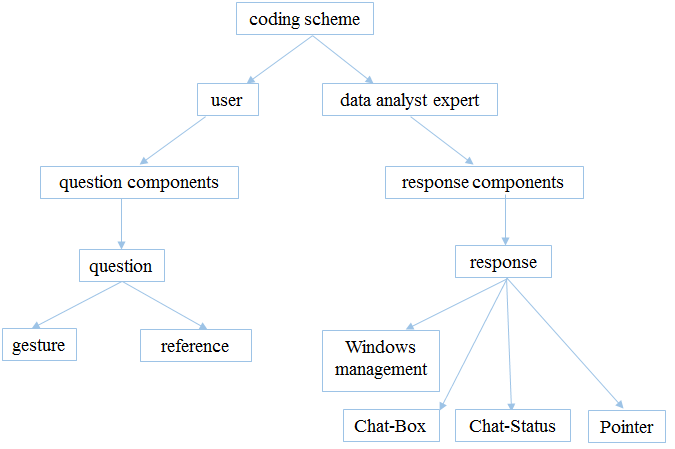
\includegraphics[width=1.0\textwidth]{coding_scheme.png}

\begin{itemize}
\item Question track corresponds to the duration of the question asked by the user. 
\item Question track begins when user starts asking question and ends when user has finished asking that question.
\item Gesture and reference tracks are single point tracks and added when they actually occur during the question.
\item Response track corresponds to the duration of the response by the data analysis expert.
\item Response track begins when data analysis expert starts processing the user question and ends when the data analysis expert completes the request (ex: new visualization is centered on screen, updates chat-box to say "sorry cannot do that", etc.).
\item Windows management, chat-box, chat-status, and pointer are single point tracks and added when they actually occur during the response.
\end{itemize}

\subsection{Annotations}
We will be annotating the question and response components as described in detail below.
\begin{itemize}

\item User - Question Component Annotations \\

\begin{tabular}{ |p{4cm}|p{5cm}|p{5cm}|  }
\hline
\multicolumn{3}{|c|}{Question} \\
\hline
Attribute& Description & Example \\
\hline
QuestionID & Enter unique identifier for the question. & Enter "Q1" for the first question, "Q2" for the second question, etc. \\
Transcription & Enter word-for-word transcription of the question. Non-words are surrounded by "*" and pauses of x-seconds are denoted [x]. & If user says "uhh (then 4 second pause) show me the (2 second pause) crime data for all four neighborhoods", then enter "*uhh* [4] show me the [2] crime data for all four neighborhoods." \\
FollowedFrom & Enter the QuestionID or VisID of the original question or visualization that generated the current question. & If the current question is independent of previous questions and visualizations, enter "null". If the user looks at visualization "1-3.png" and then asks "Can you label each line in the graph with the corresponding crime name?", then "1-3.png" generated this question, hence enter "V1-3". If the user generated the current question based on question 2, then enter "Q2". \\
\hline
\end{tabular}


\begin{tabular}{ |p{4cm}|p{5cm}|p{5cm}|  }
\hline
\multicolumn{3}{|c|}{Gesture} \\
\hline
Attribute & Description & Example \\
\hline
QuestionID & Enter unique identifier for the question. & Enter "Q1" for the first question, "Q2" for the second question, etc. \\
GestureID & Enter unique identifier for the gesture. & Enter "G1" for first gesture, "G2" for second gesture, etc. \\
Type & From the pull-down menu, select appropriate gesture type. & If user points to a line in a visualization, enter "point". \\
Target & Enter the target of the gesture. &
If one visualization: Target=VisID, 
If set of visualizations: Target = VisID,VisID, 
If a bar in visualization: Target=HistogramBarN, 
If an axis in visualization: Target=xAxisN \\
Intention & From the pull-down menu, select the intention of the gesture. What were they trying to communicate with the gesture? Indicate a visualization? Express a desire to move a visualization? & If the user points at a visualization, then select "indicate-visualization". \\

\hline
\end{tabular}


\begin{tabular}{ |p{4cm}|p{5cm}|p{5cm}|  }
\hline
\multicolumn{3}{|c|}{Reference} \\
\hline
Attribute& Description & Example \\
\hline
ReferringExpression & Enter the referring expression found from the question. & If the question is "Can I see this as a histogram?", then enter "this". If the question is "Can I see this  and that but by day of the week?", then enter "this;that". \\
GestureID & Enter the id corresponding to the Gesture track. Enter "null" if the reference was known from context and not gesture.   & Enter "G4" if reference corresponds to GestureID "G4" from Gesture track. Enter "null" if reference is known from context not any gesture. \\
ThingReferredTo & Enter the actual object being referred to. & If the question is, "Can I see this as a histogram?", and "this" points to viz "1-1.png", then enter "V1-1". If the question is "Can I see this and that but by day of the week?", and "this" points to viz "1-1.png" and "that" points to viz "1-2.png", then enter "V1-1;V1-2". \\
RefId & Enter unique identifier for the reference. & Enter "R1" for first reference, "R2" for second reference, etc. \\
ReferenceKnownFrom & From the pull-down menu, select "context" if reference is known in context or "gesture" if the reference is known from a gesture. If neither, contact the group to discuss. & If the DAE generates vis "1-5.png" and the user asks, "Can I see the same thing but for theft and battery only?", then "the same thing" refers to "1-5.png" and we know this from context, as no gesture was made. \\
\hline
\end{tabular}

\item Data analyst expert - Response Component Tracks \\

\begin{tabular}{ |p{4cm}|p{5cm}|p{5cm}|  }
\hline
\multicolumn{3}{|c|}{Response} \\
\hline
Attribute& Description & Example \\
\hline
ResponseID & Enter unique identifier for the response. & Enter "R1" for the first response, "R2" for the second response, etc. \\
ResponseToQuestion & Enter the QuestionID of the question that caused this response. & If this is a response to question "Q3", then enter "Q3". If no question is asked, then enter "null". \\
\hline
\end{tabular}

\begin{tabular}{ |p{4cm}|p{5cm}|p{5cm}|  }
\hline
\multicolumn{3}{|c|}{Windows Management} \\
\hline
Attribute& Description & Example \\
\hline
ResponseID & Enter unique identifier for the response. & Enter "R1" for the first response, "R2" for the second response, etc. \\
ResponseToQuestion & Enter the QuestionID of the question that caused this response. & If this is a response to question "Q3", then enter "Q3". If no question is asked, then enter "null". \\
Type & From the pull-down menu, select the windows management action taken by the data analysis expert. & If the data analysis expert created a new visualization and moved it to the center of the screen, then select "new-vis". If the data analysis expert moved a visualization to the side, then enter "move-vis-aside". \\
VisIDs & Enter the list of visualization ids separated by semi-colons, for each visualization that is part of this response.  Give each visualization in the visualization response an id.  Look in the Dropbox folder and match the id to the image file. & If one visualization is given, and it is called "1-1.png", then enter "V1-1". If multiple visualizations are part of the response, and they are called "1-1.png" and "1-2.png", then enter "V1-1;V1-2". \\
\hline
\end{tabular}

\begin{tabular}{ |p{4cm}|p{5cm}|p{5cm}|  }
\hline
\multicolumn{3}{|c|}{Chat-Box} \\
\hline
Attribute& Description & Example \\
\hline
ResponseID & Enter unique identifier for the response. & Enter "R1" for the first response, "R2" for the second response, etc. \\
ResponseToQuestion & Enter the QuestionID of the question that caused this response. & If this is a response to question "Q3", then enter "Q3". If no question is asked, then enter "null". \\
Type & From the drop-down menu, select the type of chat that the data analysis expert wrote. & If the data analysis expert wrote "hello!", then select "greeting". If the data analysis expert wrote "Sorry, I do not have the data.', then select "do-not-have-data". \\
Transcription & Enter the word-for-word text in the chat window. & If the chat-window text is "Yes, processing.", then enter "Yes, processing.".\\
\hline
\end{tabular}

\begin{tabular}{ |p{4cm}|p{5cm}|p{5cm}|  }
\hline
\multicolumn{3}{|c|}{Chat-Status} \\
\hline
Attribute& Description & Example \\
\hline
ResponseID & Enter unique identifier for the response. & Enter "R1" for the first response, "R2" for the second response, etc. \\
ResponseToQuestion & Enter the QuestionID of the question that caused this response. & If this is a response to question "Q3", then enter "Q3". If no question is asked, then enter "null". \\
Status & From the pull-down menu, select the chat status. & If the data analyst expert updates the chat status to "Processing", then select 'Processing".\\
\hline
\end{tabular}

\begin{tabular}{ |p{4cm}|p{5cm}|p{5cm}|  }
\hline
\multicolumn{3}{|c|}{Pointer} \\
\hline
Attribute& Description & Example \\
\hline
ResponseID & Enter unique identifier for the response. & Enter "R1" for the first response, "R2" for the second response, etc. \\
ResponseToQuestion & Enter the QuestionID of the question that caused this response. & If this is a response to question "Q3", then enter "Q3". If no question is asked, then enter "null". \\
Intention & From the drop-down menu, select the intention of the data analysis expert when the pointer is used as a response. & If the data analysis expert updates the chat-status window but the user does not see it, then the data analysis expert will use the pointer to get attention. Hence, select "get-attention". \\
\hline
\end{tabular}

\begin{tabular}{ |p{4cm}|p{5cm}|p{5cm}|  }
\hline
\multicolumn{3}{|c|}{Visualization} \\
\hline
Attribute& Description & Example \\
\hline
ResponseID & Enter unique identifier for the response. & Enter "R1" for the first response, "R2" for the second response, etc. \\
ResponseToQuestion & Enter the QuestionID of the question that caused this response. & If this is a response to question "Q3", then enter "Q3". If no question is asked, then enter "null". \\
VisIDs & Enter the list of visualization ids separated by semi-colons, for each visualization that is part of this response. Give each visualization in the visualization response an id. Look in the Dropbox folder and match the id to the image file. & If one visualization is given, and it is called "1-1.png", then enter "V1-1". If multiple visualizations are part of the response, and they are called "1-1.png" and "1-2.png", then enter "V1-1;V1-2". \\
\hline
\end{tabular}

\end{itemize}

\section{Planned Coding Scheme Extensions}
In the future, we also plan to extend our coding scheme to incorporate the following list.

\begin{itemize}
	\item Dialogue acts between the user and data analysis expert.
	\item Distinguishing between where think-aloud ends and question begins.
	\item Any activity that influences questions (such as references made) during think-aloud.
	\item Actual transcription of chat response and chat status updates.
\end{itemize}

\section{Appendix - Helpful Documents}
For annotation, helpful documents are available in Dropbox at the following location: \\
Articulate EAGER/Data collection and user study/Visualizations from user study/
\\\\
Particularly, "the real thing" contains the documents for the actual subjects in which the chart titles used for each visualization is in "full-formed English", while "the real thing 2" contains the documents for the actual subjects in which the chart titles used for each visualization is in "broken English".
\\\\
The subject documents include the videos, the actual visualizations generated, and an "approximate" transcription of the the questions asked by the user.
\end{document}
